\documentclass[12pt,letterpaper]{article}
\usepackage[utf8]{inputenc}
\usepackage[spanish]{babel}
\usepackage{graphicx}
\usepackage[left=2cm,right=2cm,top=2cm,bottom=2cm]{geometry}
\usepackage{graphicx} % figuras
% \usepackage{subfigure} % subfiguras
\usepackage{float} % para usar [H]
\usepackage{amsmath}
%\usepackage{txfonts}
\usepackage{stackrel} 
\usepackage{multirow}
\usepackage{enumerate} % enumerados
\renewcommand{\labelitemi}{$-$}
\renewcommand{\labelitemii}{$\cdot$}
% \author{}
% \title{Caratula}
\begin{document}

% Fancy Header and Footer
% \usepackage{fancyhdr}
% \pagestyle{fancy}
% \cfoot{}
% \rfoot{\thepage}
%

% \usepackage[hidelinks]{hyperref} % CREA HYPERVINCULOS EN INDICE

% \author{}
\title{Caratula}

\begin{titlepage}
\begin{center}
\large{UNIVERSIDAD PRIVADA DE TACNA}\\
\vspace*{-0.025in}
\begin{figure}[htb]
\begin{center}

\end{center}
\end{figure}
\begin{center}
    
\includegraphics[width=6cm, height=5cm]{img/upt.jpg}  
\end{center}

\vspace*{0.15in}
INGENIERIA DE SISTEMAS  \\

\vspace*{0.5in}
\begin{large}
TITULO:\\
\end{large}

\vspace*{0.1in}
\begin{Large}
\textbf{Desarrollo de Solución de Mejora de RandyStore} \\
\end{Large}

\vspace*{0.3in}
\begin{Large}
\textbf{CURSO:} \\
\end{Large}

\vspace*{0.1in}
\begin{large}
BASE DE DATOS II\\
\end{large}

\vspace*{0.3in}
\begin{Large}
\textbf{DOCENTE:} \\
\end{Large}

\vspace*{0.1in}
\begin{large}
Ing. Patrick Cuadros Quiroga\\
\end{large}

\vspace*{0.2in}
\vspace*{0.1in}
\begin{large}
Integrantes: \\
\begin{flushleft}

Mej\'ia Rodriguez, Julio Oliver         	\hfill	(2010037899) \\
Paredes Catacora, Randi Angel   	\hfill	(2013047246) \\
Herrera Amezquita, Derian Francisco		\hfill	(2017059489) \\
Lipa Calabilla, Abraham		\hfill	(2019064039) \\

\end{flushleft}
\end{large}
\end{center}

\end{titlepage}



\tableofcontents % INDICE
\thispagestyle{empty} % INDICE SIN NUMERO
\newpage
\setcounter{page}{1} % REINICIAR CONTADOR DE PAGINAS DESPUES DEL INDICE


\begin{center}
    \textbf{\Large Resumen}  
\end{center}

El presente proyecto , desarrollo de una sistema de control de clientes, personal e
inventario del gimnasio Randys busca  contribuir automatizar los procesos del area 
de ventas de productos deportivos.
Tambien busca llevar un control de los clientes y de el personal con el que cuenta la 
tienda. 
\\
\begin{center}
    \textbf{\Large Abstract}
\end{center}

The present project, development of a control system for clients, personnel and
Randys gym inventory seeks to help automate processes in the area
sales of sports products.
It also seeks to keep track of customers and staff with whom the company has
store.

\section{Introduccion} 

\section{Titulo} 

Sistema de control de inventario y personal RandyStore.

\section{Autores} 
\begin{itemize}
    \item Mej\'ia Rodriguez, Julio Oliver    
    \item Paredes Catacora, Randi Angel 
    \item Herrera Amezquita, Derian Francisco
    \item Lipa Calabilla, Abraham
\end{itemize}

\section{Planteamiento del problema} 
    \subsection{Problema}
    La tienda RandyStore no cuenta con un control sobre los productos y ventas que realizan sus empleados   
    por lo que estos guardan infromacion en lugares no muy confiables como cuadernos los cuales se pueden dañar 
    y afectar a la tienda.
    \subsection{Justificación}
    La implementación del sistema RandyStore tiene una gran importancia debido a que va a mejorar notablemente la calidad de los datos de ventas generadas por el personal de ventas para mejorar el control de los registros de los productos y de las ventas, así como la seguridad de los datos.
    \subsection{Alcance}
    El alcance del proyecto sera a el gerente y los empleados que trabajan en la tienda para que puedan monitoriar
    y/o controlar los ingresos y ventas de productos relacionados a la tienda.
\section{Objetivos}
    \subsection{General}
    Ayudar a llevar un control sobre el stock de la tienda y mejorar el control de las ventas realizadas por el personal de ventas de la tienda.
    \subsection{Específicos}
    \begin{itemize}
        \item Añadir seguridad a el sistema mediante un login.
        \item Control sobre productos ,empleados y clientes.
    \end{itemize}

\section{Referencias Teoricas}

\subsection{Net Core}

NET Core es un Framework informático administrado, gratuito y de código abierto para los sistemas operativos Windows, Linux y MacOS. Es un sucesor multiplataforma de .NET Framework. El proyecto es desarrollado principalmente por Microsoft bajo la Licencia MIT.

\subsection{ASP.NET Core}

ASP.NET Core es un framework web gratis de código abierto y con un mayor rendimiento que ASP.NET, desarrollado por Microsoft y la comunidad. Es un framework modular que se ejecuta completo tanto en el.NET Framework de Windows como en multiplataforma. NET Core.

\subsection{MongoDB}

MongoDB es un sistema de base de datos NoSQL, orientado a documentos y de código abierto.

En lugar de guardar los datos en tablas, tal y como se hace en las bases de datos relacionales, MongoDB guarda estructuras de datos BSON (una especificación similar a JSON) con un esquema dinámico, haciendo que la integración de los datos en ciertas aplicaciones sea más fácil y rápida. 

\subsection{API}

La interfaz de programación de aplicaciones, conocida también por la sigla API, en inglés, application programming interface, es un conjunto de subrutinas, funciones y procedimientos que ofrece cierta biblioteca para ser utilizado por otro software como una capa de abstracción.

\subsection{Controller}

Un Controller o Controlador es una clase que deriva de la clase ControllerBase y es usado por una Web API para manejar las solicitudes.

\subsection{Inyección de dependencias}

Es un patrón de diseño orientado a objetos, en el que se suministran objetos a una clase en lugar de ser la propia clase la que cree dichos objetos. Esos objetos cumplen contratos que necesitan nuestras clases para poder funcionar (de ahí el concepto de dependencia).

\section{ Desarrollo de Solución de Mejora}

\subsection{Casos de Uso de la aplicación}

\begin{center}
    \includegraphics[width=18cm, height=10cm]{img/índice3.jpg}  
\end{center}

\subsection{Diagrama de Arquitectura de la aplicación}

\begin{center}
    \includegraphics[width=14cm, height=4cm]{img/índice4.jpg}  
\end{center}

\subsection{Diagrama de Clases de la aplicación}

\begin{center}
    \includegraphics[width=18cm, height=10cm]{img/casos2.png}  
\end{center}

\section{Diccionario de datos}

Tabla de cargos de empleados
\begin{center}
    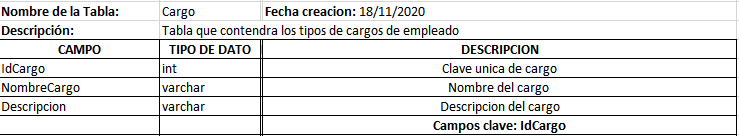
\includegraphics[width=14cm, height=3cm]{img/cargo.png}  
\end{center}
Tabla de categorias de producto
\begin{center}
    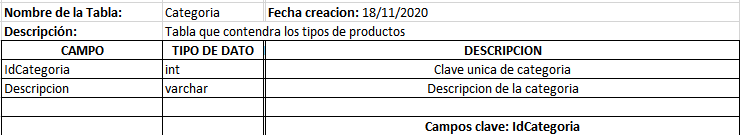
\includegraphics[width=14cm, height=3cm]{img/categoria.png}  
\end{center}
\newpage
Tabla de cliente
\begin{center}
    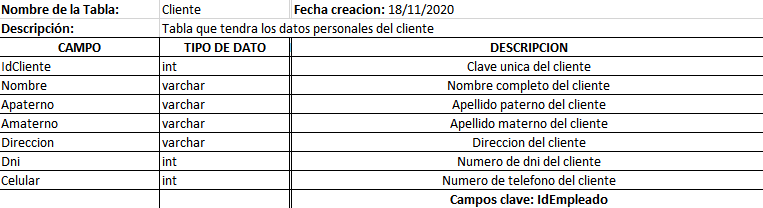
\includegraphics[width=14cm, height=4cm]{img/cliente.png}  
\end{center}
Tabla de comprobante
\begin{center}
    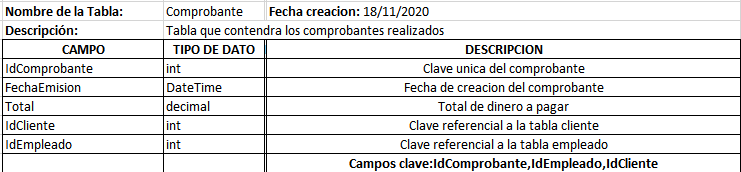
\includegraphics[width=14cm, height=4cm]{img/comprobante.png}  
\end{center}
Tabla del detalle del comprobante
\begin{center}
    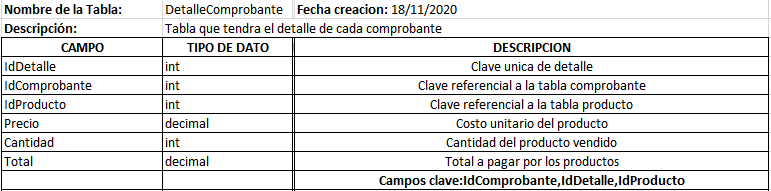
\includegraphics[width=14cm, height=4cm]{img/detalle.png}  
\end{center}
Tabla del empleado
\begin{center}
    \includegraphics[width=14cm, height=5cm]{img/empleado.png}  
\end{center}
\newpage
Tabla del producto
\begin{center}
    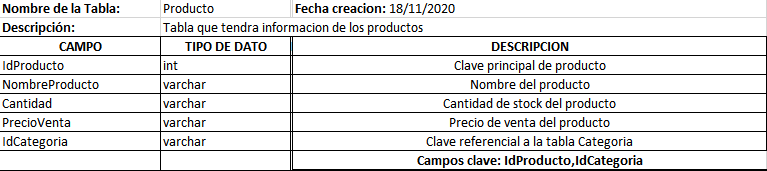
\includegraphics[width=14cm, height=4cm]{img/producto.png}  
\end{center}

\section{Cadena de conexion }

Guardamos los datos de conexión de MongoDB en el fichero appsettings.json. Guardamos el servidor, la base de datos y la colección en que se guardará.

\begin{center}
    \includegraphics[width=14cm, height=4cm]{img/índice.jpg}  
\end{center}

En Startup.cs, configuramos el servicio con la configuración en el json.

\begin{center}
    \includegraphics[width=14cm, height=4cm]{img/índice2.jpg}  
\end{center}

En el controlador, declaramos dos operaciones: Get (que devuelve todos los registros de Ingreso) y Post (que permite registrar un ingreso).

\begin{center}
    \includegraphics[width=14cm, height=4cm]{img/índice5.jpg}  
\end{center}

\end{document}
